
\section{Discussion}
\label{sec:discussion}

The mechanism above shifts attention from prompts to the regions of reasoning states they induce. An input is useful when the student's rollouts reach regions where the teacher can provide useful supervision. Stating a problem is only one way to reach them. This view raises two broader questions: how much task content must the input itself contain, and why does the same one-shot setting behave differently under OPD and RLVR? We discuss these questions through content-light and off-domain inputs, followed by a controlled comparison with one-shot RLVR.

\subsection{Inputs as State Generators}
\label{sec:template}

The state-generator view suggests that task content may be unnecessary if an input still induces trajectories that the teacher can supervise. We stress-test this prediction with an empty user turn ending in \texttt{<think>}, the same template with a simple domain system prompt, and general-domain queries from WildChat~\citep{zhao2024wildchat} (Figure~\ref{fig:template-examples}). The WildChat set contains \(192{,}824\) predominantly English queries from general conversation, creative writing, role-playing, and rewriting. Conservative heuristics label only \(0.17\%\) as mathematics-related and \(2.63\%\) as code-related.

\begin{figure}[t]
\centering
\begin{minipage}[t]{0.485\textwidth}
\begin{tplbox}{(a) Base template}
\begin{tplinput}
\ttfamily\scriptsize\raggedright \tplctrl{<|begin\_of\_sentence|>}\tplrole{<|User|>}\tplthink{<think>}\tplesc{\textbackslash n}
\end{tplinput}
\end{tplbox}
\end{minipage}\hfill
\begin{minipage}[t]{0.485\textwidth}
\begin{tplbox}{(b) System template --- Code}
\begin{tplinput}
\ttfamily\scriptsize\raggedright \tplctrl{<|begin\_of\_sentence|>}Solve competitive programming problems. Read from stdin, write to stdout.\tplrole{<|User|>}\tplthink{<think>}\tplesc{\textbackslash n}
\end{tplinput}
\end{tplbox}
\end{minipage}
\\[4pt]
% {\scriptsize\tplctrl{\ttfamily control token}\quad\tplrole{\ttfamily role token}\quad\tplthink{\ttfamily reasoning token}\quad\tplesc{\ttfamily literal newline}\quad{\ttfamily instruction text}}
\caption{The two content-light templates used as OPD training inputs.}
\label{fig:template-examples}
\end{figure}

\begin{figure}[t]
\centering
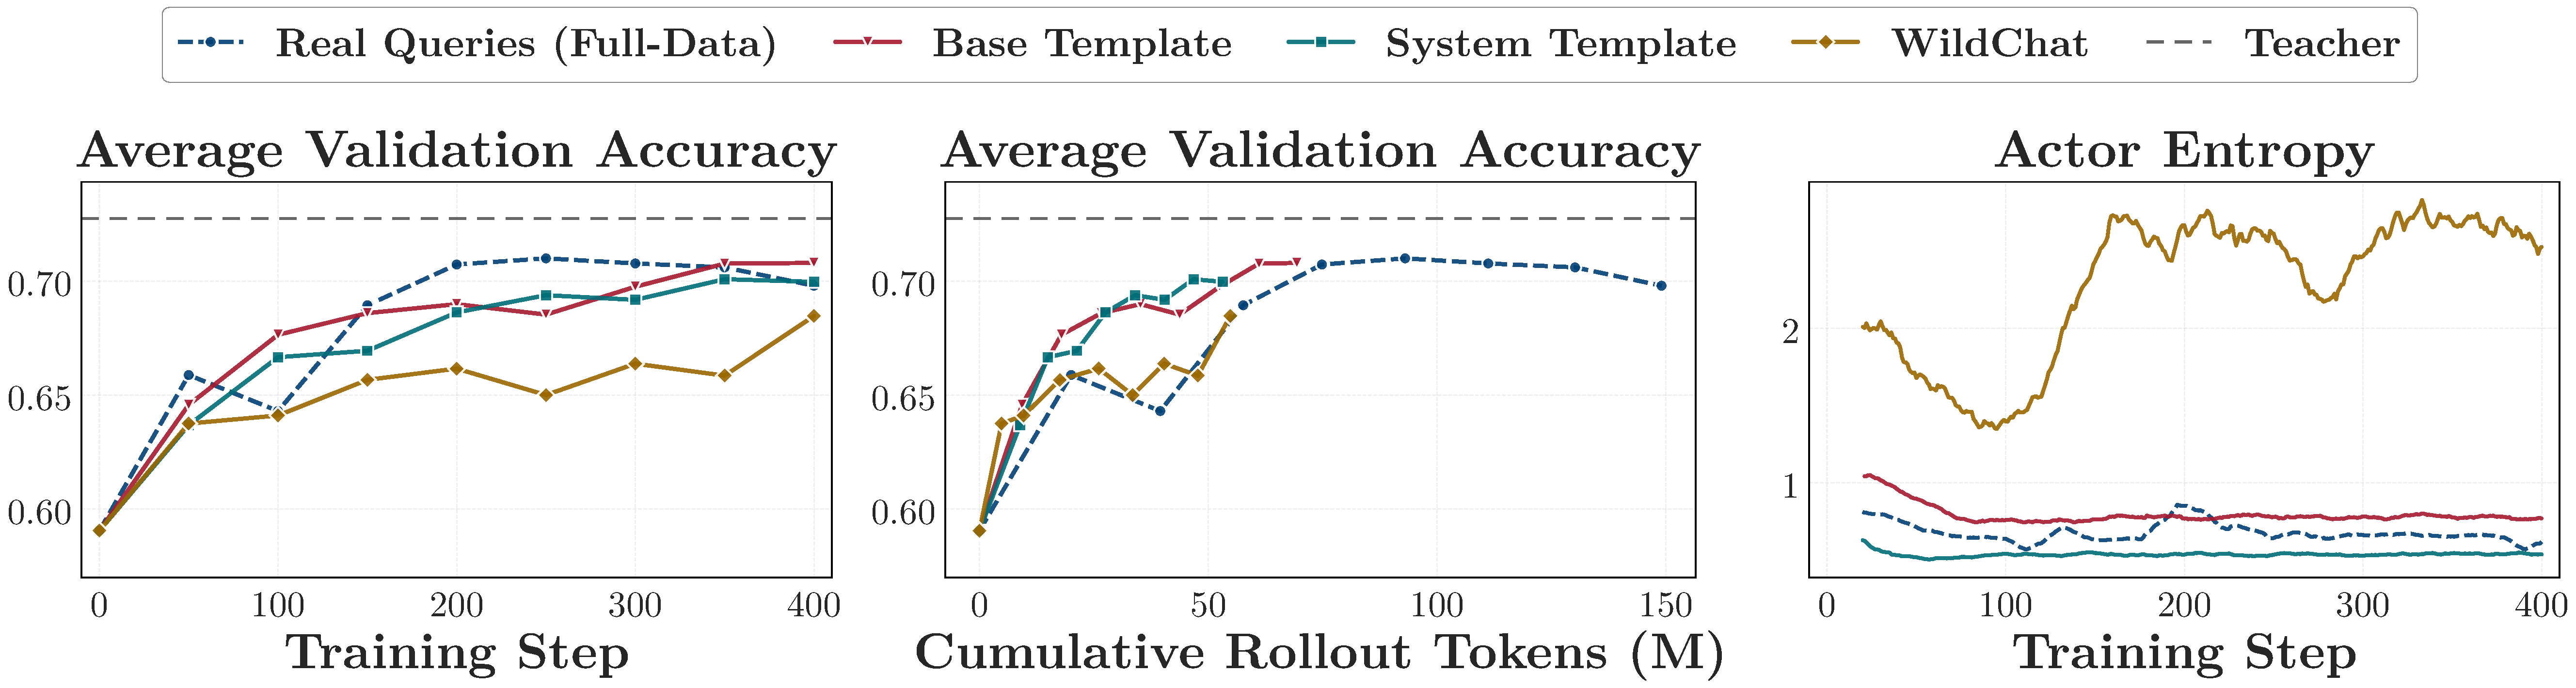
\includegraphics[width=\textwidth]{figures/7_template_wildchat.pdf}
\caption{
Validation accuracy and actor entropy for mathematics OPD trained on the real training set, on a content-light template, or on general-domain WildChat queries.
}
\label{fig:template-wildchat}
\end{figure}

\paragraph{Content-light and off-domain inputs can still induce useful states.}
% \paragraph{The input does not have to state a problem, even domain.}
All three conditions track the real-query baseline, which lifts the three-benchmark average from \(59.1\) to \(69.8\), and all three reach that level on a third to a half of its rollout tokens (Figure~\ref{fig:template-wildchat}). Code generation gives the same picture (Appendix~\ref{app:template-code}). 
However, the requirement is not empty: a scaffold that closes the block at once, \texttt{<think>\textbackslash n}\allowbreak\texttt{</think>\textbackslash n}, collapses into short meta-level replies we cannot train on.
These results do not imply that task content is generally dispensable. They show that content is not the only source of useful signal in OPD. An input also acts as a state generator, and even content-light or off-domain inputs can sometimes lead the student to states that support useful teacher supervision. Explicit domain content changes final performance by about one point in these experiments. This provides a complementary view of OPD data efficiency. Data quality depends not only on the problems being collected, but also on the state regions they induce and the teacher targets available there.

\subsection{Relation to One-Shot RLVR}
\label{sec:opd-vs-rlvr}

One-shot OPD and one-shot RLVR~\citep{wang2025oneshot} share the same surface phenomenon that a single query supports continued improvement over hundreds of updates in OPD and over a thousand updates in RLVR. The source of learning is different. OPD receives a teacher target at every visited state, while RLVR receives a verifiable outcome for each trajectory. We compare them on the same medium query to isolate this difference (Figure~\ref{fig:opd-vs-rlvr}).

\begin{figure}[t]
\centering
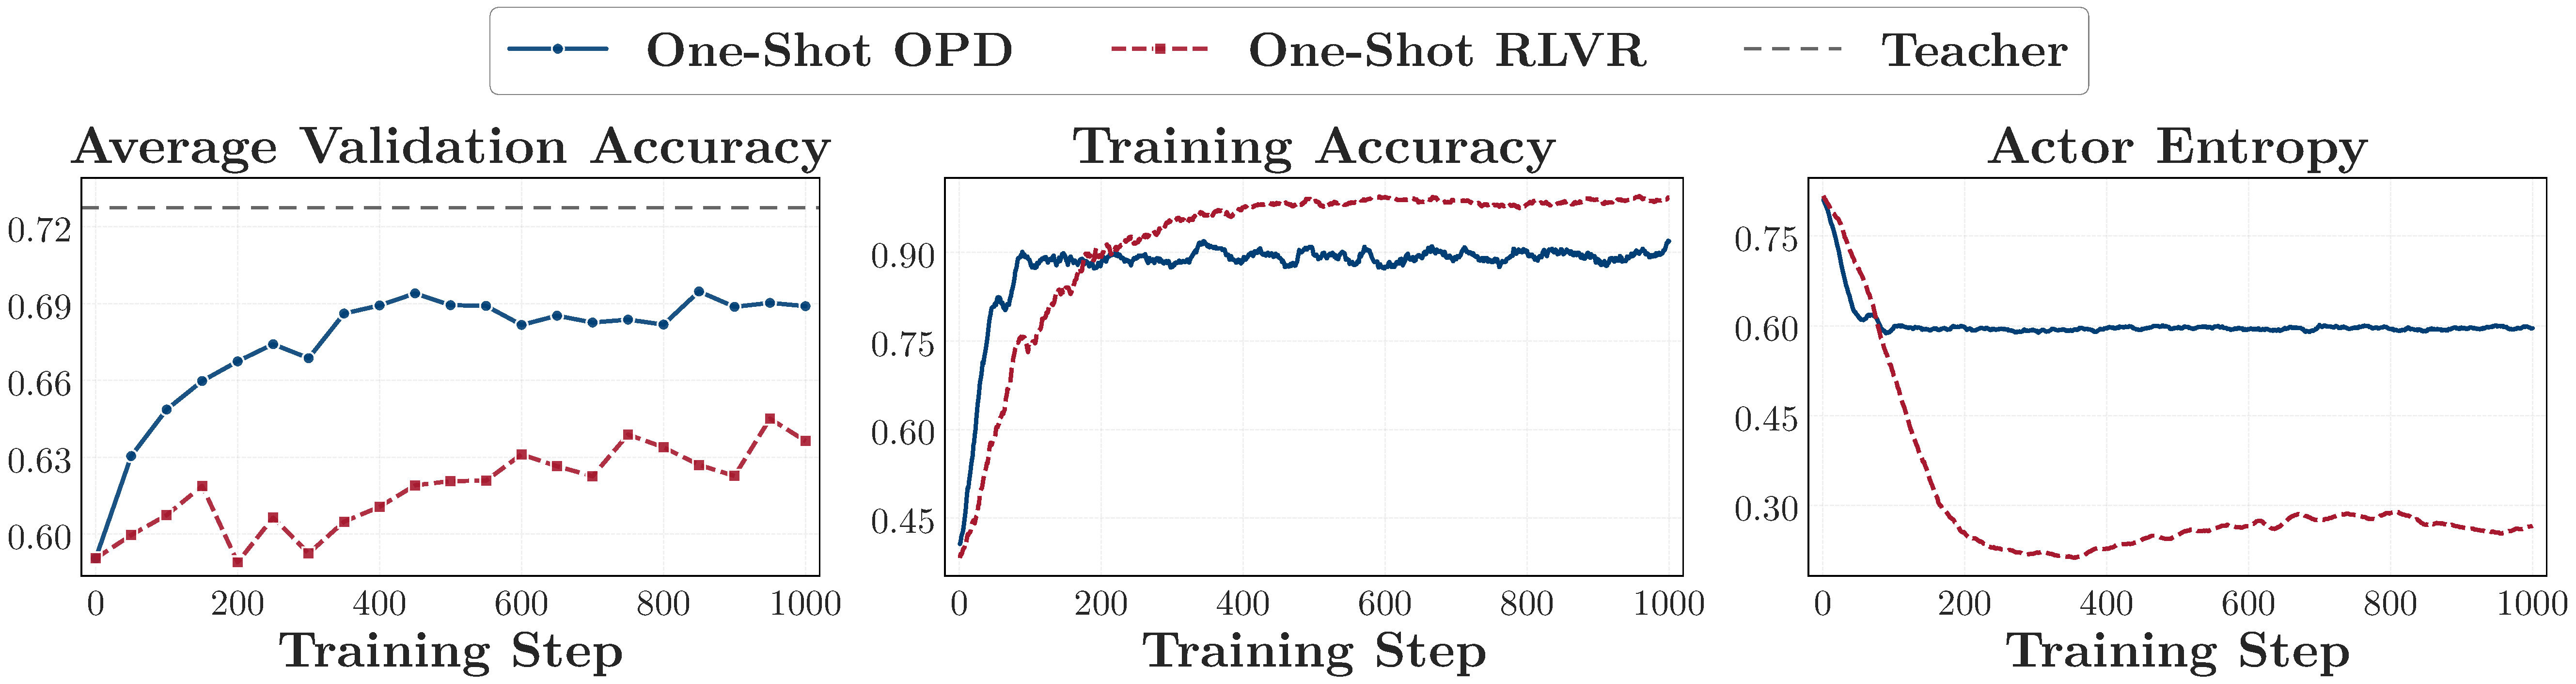
\includegraphics[width=\textwidth]{figures/7_opd_vs_rlvr.pdf}
\caption{
Validation accuracy and training dynamics for one-shot OPD and one-shot RLVR on the same query. Both take a batch of \(64\) queries per step. RLVR draws \(8\) rollouts per query and scores each by outcome under GRPO. OPD draws \(1\) and scores every sampled token against the teacher. Training accuracy is the fraction of rollouts that solve the training query.
% which RLVR optimizes and OPD only measures.
}
\label{fig:opd-vs-rlvr}
\end{figure}

\paragraph{Useful inputs differ across objectives.}
RLVR updates from trajectory outcomes. Its training input must therefore define a task whose sampled outcomes can be verified. The outcomes must also vary enough to produce a useful advantage. OPD instead updates from the teacher--student gap at each visited state. It can receive useful signal whenever a prompt leads to trajectories that expose such gaps. The value of an OPD input is therefore not tied directly to verifiability or difficulty. Our results further show that even weak domain alignment can work in the settings we study. Coverage of the induced state regions still matters (Section~\ref{sec:data}), but obtaining such coverage is less restrictive than obtaining tasks with verifiable outcomes.

\paragraph{OPD extracts more signal from the same query.}
Both algorithms obtain fresh rollouts from the training query at every step. Over \(1000\) steps, OPD closes \(72\%\) of its gap to the teacher. Its gain in validation accuracy is more than twice that of RLVR. This advantage remains when the two methods are matched by rollout tokens rather than training steps (Figure~\ref{fig:opd-vs-rlvr}).

The RLVR signal weakens as the model learns to solve the training query. Its groups soon become nearly unanimous, which leaves no advantage under GRPO. OPD does not depend on variation in trajectory outcomes. It can continue learning from local teacher--student gaps after the query is solved, although these gaps gradually shrink. One-shot RLVR is therefore limited by the outcome variation available from its query. One-shot OPD is instead limited by how quickly it absorbs dense teacher supervision, as shown in Sections~\ref{sec:data} and~\ref{sec:algorithm}. The objectives also imply different ceilings. RLVR is not tied to a teacher's distribution, while OPD is trained to match one.
